\documentclass[a4paper,12pt]{article}

% Set margins
\usepackage[hmargin=2.5cm, vmargin=2cm]{geometry}

\frenchspacing

% Language packages
\usepackage[utf8]{inputenc}
\usepackage[T1]{fontenc}
\usepackage[magyar]{babel}

% AMS
\usepackage{amssymb,amsmath}

% Graphic packages
\usepackage{graphicx}

% Colors
\usepackage{color}
\usepackage[usenames,dvipsnames]{xcolor}

% Enumeration
\usepackage{enumitem}

% Links
\usepackage{hyperref}

\pagestyle{empty}

\begin{document}

\begin{center}
\Large \bf Képfeldolgozás -- Vizsga feladatok
\end{center}

\vskip 5mm

\section{Képfeldolgozási szoftverek}

\textit{Soroljon fel legalább 5 olyan szoftveres eszközt, amely a képfeldolgozási problémák megoldása során hasznos lehet! Jellemezze ezeket röviden!}

\bigskip

\noindent Képfeldolgozáshoz például az alábbi szoftvereket használhatjuk.

\begin{itemize}
	\item \textit{OpenCV}: Nyílt, szabványos gépi látásos (\textit{Computer Vision}) függvénykönyvtár C++ nyelvhez. Python wrapper elérhető hozzá.
	\item \textit{NumPy}: Numerikus függvénykönyvtár Python-hoz. A lineáris algebrai eszközöket (vektorokat, mátrixokat és műveleteiket) biztosítja.
	\item \textit{Matplotlib}: Függvényábrázoló függvénykönyvtár Python-hoz. A NumPy típusait tudja használni.
	\item \textit{Scikit Learn}: Gépi tanuláshoz használható függvénykönyvtár.
	\item \textit{Jupyter}: Interaktív, munkafüzet alapú fejlesztést segítő keretrendszer. Többségében Python programozási nyelvvel használják, de más nyelvekhez is elérhető.
	\item \textit{GIMP}: Nyílt forráskódú képszerkesztő program.
\end{itemize}

Említhetők például még a következők is: Seaborn, PhotoShop, PyTorch, TensorFlow, SciPy, Pillow/PIL.

\section{Képformátumok}

\textit{Mutassa be a képek tárolási formátumainak egy elterjedt osztályozási módját! Sorolja fel az elterjedt formátumokat!}

\bigskip

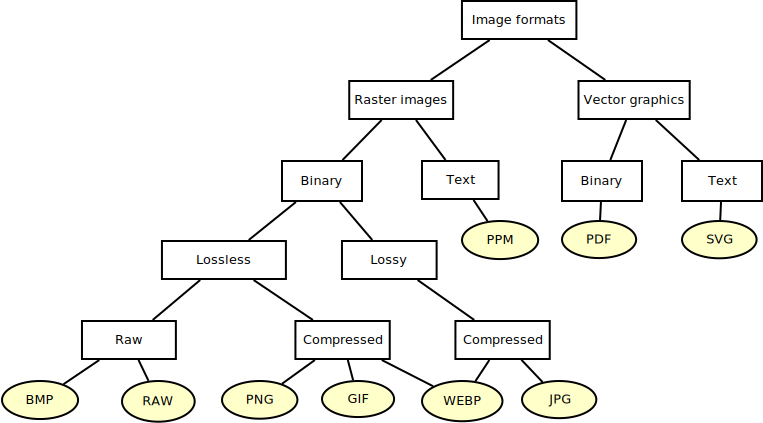
\includegraphics[width=\textwidth]{images/image_formats.png}

\begin{itemize}
	\item BMP: \textit{BitMap}, egyszerű, bittérképes formátum.
	\item RAW: Nyers képformátum. Főként fotózásban használják.
	\item PNG: \textit{Portable Network Graphics}, az Internet képformátumának hozták létre.
	\item GIF: \textit{Graphics Interchange Format}, főként kisebb méretű, animált, helyenként átlátszó képekhez.
	\item WebP: Az Internet következő preferált képformátuma.
	\item JPG: \textit{Joint Photographic Experts Group}, fényképekre kifejlesztett formátum.
	\item PPM: \textit{Portable PixMap}, egyszerű raszteres formátum.
	\item PDF: \textit{Portable Document Format}, bináris képformátumnak tekinthető.
	\item SVG: \textit{Scalable Vector Graphics}, XML alapú vektorgrafikus képformátum.
\end{itemize}


\section{Szürkeárnyalatos leképzés}

\textit{Mutasson be legalább 3 olyan számítási módot, amely segítségével egy színes (RGB színtérbeli) képből szürkeárnyalatosat kaphatunk!}

\bigskip

\noindent A leképzés egy $\mathbb{R}^3 \rightarrow \mathbb{R}$ (pontosabban $[0, 1]^3 \rightarrow [0, 1]$) leképzés formájában írható fel. Néhány gyakori megközelítés:

\begin{itemize}
	\item $f(r, g, b) = \dfrac{r + g + b}{3}$.
	\item $f(r, g, b) = \max(r, g, b)$.
	\item $f(r, g, b) = \dfrac{\min(r, g, b) + \max(r, g, b)}{2}$.
\end{itemize}

\section{Árnyalatokhoz kötődő színterek}

\textit{Mutassa be a HSI, HSV és HSL színtereket!}

\bigskip

\noindent \url{https://en.wikipedia.org/wiki/HSL_and_HSV}

\section{Zaj típusok}

\textit{Soroljon fel legalább 5 zaj típust, és hogy mi okozhatja!}

\bigskip

\noindent Gyakran előforduló zajtípusok például az alábbiak:

\begin{itemize}
	\item Pontszerű zaj: származhat például a képalkotó eszköz (például CCD szenzor) hibájából.
	\item Fehér zaj: származhat a megvilágítás egyenetlenségéből, különféle sugárzások okozta hatásból.
	\item Elmosódott részek: okozhatja a rosszul beállított fókusz, mélységélesség.
	\item Színtérből adódó zaj: a közeg színe vagy a színes megvilágítás okozhatja.
	\item Túlexponálás: a túlságosan hosszú expozíciós idő okozza.
	\item Perspektív torzítás: a kamerák fizikai kialakításából adódik.
	\item Elmosódásos zaj: az exponálás közben bemozdult kamera okozhatja.
	\item Mintavételezési, tömörítési zaj: például a JPG (veszteséges) tömörítésnél figyelhető meg.
	\item Hiányzó, kitakart képrészek: a rossz kamerabeállítások, útban lévő objektumok okozhatják.
\end{itemize}

\section{Hisztogram számítása}

\textit{Jelölje az $I \in [0, 255]^{n \times m}$ egy szürkeárnyalatos kép intenzitás mátrixát! Írja le (matematikai formulák és/vagy pszeudókód) segítségével a hisztogram számítási módját!}

\bigskip

\noindent Jelölje a hiszgramot a $h \in \mathbb{Z}^{256}$ vektor! Feltételezzük, hogy az indexeket 0-tól indítjuk. Ekkor a $h$ értékét a következőképpen számíthatjuk ki:
$$
h[k] = |\{(x, y) \in I : I[x, y] = k\}|.
$$

\noindent Pszeudó kód:

\begin{align*}
&\text{CALC\_HISTOGRAM}(I, @h) \\
&\text{// Input}: I \in [0, 255]^{n \times m} \\
&\text{// Output}: h \in \mathbb{Z}^{256} \\
&\text{FOR } k \leftarrow 0 \text{ TO } 255 \text{ DO} \\
&\quad h[k] \leftarrow 0 \\
&\text{FOR } i \leftarrow 1 \text{ TO } n \text{ DO} \\
&\quad \text{FOR } j \leftarrow 1 \text{ TO } m \text{ DO} \\
&\quad\quad h[I[i, j]] \leftarrow h[I[i, j]] + 1 \\
&\text{RETURN}(h) \\
\end{align*}

\section{Hisztogram műveletek}

\textit{Mutassa be a hisztogram széthúzás és a hisztogram kiegyenlítés műveletét!}

\bigskip

\noindent A hisztogram széthúzás (\textit{histogram stretching}) során arra törekszünk, hogy az eredeti intenzitástartományt a teljes (jellemzően $[0, 255]$) tartományra húzzuk szét. Az új $I'$ intenzitást az $I$ intenzitásból a következőképpen számíthatjuk ki:
$$
I' = \dfrac{I - I_{\min}}{I_{\max} - I_{\min}} \cdot 255,
$$
ahol az $I_{\min}$ a képen lévő minimális, az $I_{\max}$ pedig a képen lévő maximális intenzitást jelöli.

A hisztogram kiegyenlítés (\textit{histogram equalization}) során arra törekszünk, hogy a transzformációt követően az intenzitások eloszlása minél közelebb legyen az egyenletes eloszláshoz.

\section{Lineáris konvolúció}

\textit{Mutassa be a kernel mátrix segítségével végrehajtható lineáris konvolúciós szűrő működését!}

\bigskip

\noindent Jelölje a lineáris konvolúciós szűrő kernelét az alábbi mátrix:
$$
g \in \mathbb{R}^{(2k + 1) \times (2k + 1)}.
$$
A lineáris konvolúciót diszkrét esetben a következő számítással adhatjuk meg:
$$
(f * g)(x, y) = \sum_{i=-k}^{k} \sum_{j=-k}^{k}
f(x + j, y + i) \cdot g(j, i),
$$
ahol $f$ a kép pontbeli intenzitását írja le, a $g$ pedig a konvolúciós kernelt.

\section{Gauss szűrő}

\textit{Mit nevezünk Gauss szűrő? Adjon rá egy lineáris konvolúciós közelítést!}

\bigskip

\noindent A Gauss szűrés egy olyan konvolúciós eljárást jelöl, melyben a konvolúciós kernel a normális eloszlás görbéjét közelíti. Tetszőleges dimenzióban elvégezhető. Képek esetében ez a kétváltozós normális eloszlás haranggörbéjét jelenti (mint felület közelítését).

Gauss szűrőhöz konvolúciós kernelnek például a következő mátrixot használhatjuk:
$$
g = \dfrac{1}{16}
\begin{bmatrix}
	1 & 2 & 1 \\
	2 & 4 & 2 \\
	1 & 2 & 1 \\
\end{bmatrix}.
$$

\section{Medián szűrő}

\textit{Mutassa be a medián szűrú működését! Írja le a módszer néhány fontosabb jellemzőjét!}

\bigskip

\noindent A medián szűrő egy nemlineáris szűrő. A nevét onnan kapta, hogy a konvolúció során használt kernelhez tartozó értékeket sorba rendezzük, majd a középső elemet (a mediánt) választjuk.

\begin{itemize}
	\item A módszer előnye, hogy nem ad a képhez új intenzitást.
	\item Nagyon jól kezeli a pontszerű zajokat.
	\item Hátránya, hogy a rendezés miatt számításigényes.
\end{itemize}

\section{Élkiemelés}

\textit{Hogyan becsülhetjük, hogy hol van egy (szürkeárnyalatos) képen él? Adjon rá konkrét, lineáris konvolúciós közelítő módszert!}

\bigskip

\noindent Az éleket például a pontbeli gradienssel, annak nagyságával becsülhetjük. Jelölje $I \in \mathbb{R}^{n \times m}$ az intenzitásmátrixot. Ekkor a gradiens a
$$
\nabla I(x, y) =
\left[
\dfrac{\partial I(x, y)}{\partial x},
\dfrac{\partial I(x, y)}{\partial y}
\right]
$$
alakban írható föl.

Ennek egy numerikus, lineáris konvolúciós közelítése a Sobel operátor, amelynek kernelei:
$$
G_x = \begin{bmatrix}
	-1 & 0 & +1 \\
	-2 & 0 & +2 \\
	-1 & 0 & +1 \\
\end{bmatrix}, \quad
G_y = \begin{bmatrix}
	+1 & +2 & +1 \\
	0 & 0 & 0 \\
	-1 & -2 & -1 \\
\end{bmatrix}.
$$

\section{Lokális küszöbölés}

\textit{Adjon egy egyszerű példát adaptív, lokális küszöbölési algoritmusra!}

\bigskip

\noindent Lokális küszöböléshez használhatjuk például az alábbi, egyszerű algoritmust.

\begin{itemize}
\item Minden képponthoz határozzuk meg az adott képponttól egy adott távolságon belül elérhető képpontok halmazát.
\item Számítsuk ki ezen képpontok átlagát, amelyet lokális köszöbértékként használhatunk.
\end{itemize}

\end{document}
